%%%%% Don't Make Changes Below Here %%%%%
\documentclass{article}\usepackage[utf8]{inputenc}\usepackage[margin=0.4cm,top=0.4cm,bottom=0.4cm]{geometry}\usepackage[usenames,dvipsnames,svgnames,table]{xcolor}\usepackage{calligra}\usepackage{tikz}\usetikzlibrary{matrix,fit,chains,calc,scopes}\usepackage{tcolorbox}\tcbuselibrary{skins}\tcbset{Baystyle/.style={sharp corners,enhanced,boxrule=6pt,colframe=Aquamarine,height=\textheight,width=\textwidth,borderline={8pt}{-11pt}{},}}\usepackage{amsmath,amssymb,amsthm,tikz,tkz-graph,color,chngpage,soul,hyperref,csquotes,graphicx,floatrow,listings}\newcommand*{\QEDB}{\hfill\ensuremath{\square}}\newtheorem*{prop}{Proposition}\renewcommand{\theenumi}{\alph{enumi}}\usepackage[shortlabels]{enumitem}\usetikzlibrary{matrix,calc}\MakeOuterQuote{"}\newtheorem{theorem}{Theorem} \usetikzlibrary{shapes} \usepackage{lipsum}\usepackage{tabularx,ragged2e,booktabs,caption}\tcbuselibrary{breakable}\newenvironment{yframed}{\begin{tcolorbox}[breakable,colback=gray!3,title after break={\textit{\color{red}Solution (cont.)}},colbacktitle=gray!3, coltitle=black,titlerule=-1pt] }{\end{tcolorbox}}\newtcolorbox{mybox}{colback=black!15!white, colframe=white,arc=12pt}\newtcolorbox{myboxot}{colback=green!15!white, colframe=white,arc=12pt,width=100pt, height=27pt}\newtcbox{\mylib}{enhanced,boxrule=0pt,top=0mm,bottom=0mm,right=0mm,left=4mm,arc=4pt,boxsep=9pt,before upper={\vphantom{dlg}},colframe=green!50!black,coltext=green!25!black,colback=green!10!white,overlay={\begin{tcbclipinterior}\fill[green!75!blue!50!white] (frame.south west)rectangle node[text=white,font=\sffamily\bfseries\tiny,rotate=90] {Problem} ([xshift=4mm]frame.north west);\end{tcbclipinterior}}}\newtcbox{\mylibot}{enhanced,boxrule=0pt,top=0mm,bottom=0mm,right=0mm,arc=4pt,boxsep=9pt,before upper={\vphantom{dlg}},colframe=green!50!black,coltext=green!25!black,colback=green!10!white,overlay={\begin{tcbclipinterior}\fill[red!75!blue!50!white] (frame.south west)rectangle node[text=white,font=\sffamily\bfseries\tiny,rotate=90] {Other} ([xshift=4mm]frame.north west);\end{tcbclipinterior}}}
\def\Title{\begin{tcolorbox}[Baystyle,]{\begin{center}\vspace*{0.14\textheight}
{\rule{\textwidth}{1.6pt}\vspace*{-\baselineskip}\vspace*{2pt}}
\rule{\textwidth}{0.4pt}\\[0.2\baselineskip]{\fontsize{45}{45}\scshape CS 170: Efficient Algorithms and \\[-0.3\baselineskip] Intractable Problems \\[0.2\baselineskip] \calligra Spring 2017 \\[0.2\baselineskip]}
{\rule{\textwidth}{0.4pt}\vspace*{-\baselineskip}\vspace{3.2pt}}
\rule{\textwidth}{1.6pt}\\[\baselineskip]\vspace{0.05\textheight}{{\fontsize{45}{45}\scshape$\bullet$\\ {Homework 2}\\\vspace*{0.01\textheight} }{{\fontsize{18}{18}\scshape{Due on Tuesday, Februrary 7th, 2017 at 11:59am\\}}}\fontsize{45}{45}\scshape$\bullet$  \\}\vspace*{0.1\textheight}{\fontsize{12}{12}\calligra Solutions by\\}{\fontsize{28}{28}\scshape \Name \\}\vspace*{0.01\textheight}{\fontsize{12}{12}\scshape \SID} \\\vspace*{0.05\textheight}{\fontsize{12}{12}\calligra In collaboration with\\}\vspace*{0.01\textheight}{\fontsize{12}{12}\scshape \Collabs} \\\vspace*{0.05\textheight}\end{center}}\end{tcolorbox}\newgeometry{margin=0.75in}}\def\BeginSolution{\begin{yframed}\textbf{\color{red}Solution }}\def\EndSolution{\end{yframed}}
\usepackage{algorithm}\usepackage[noend]{algpseudocode}\makeatletter\def\BState{\State\hskip-\ALG@thistlm}\makeatother\def\T{\indent}\def\star{\bigstar}
\usetikzlibrary{arrows}
\def\graph{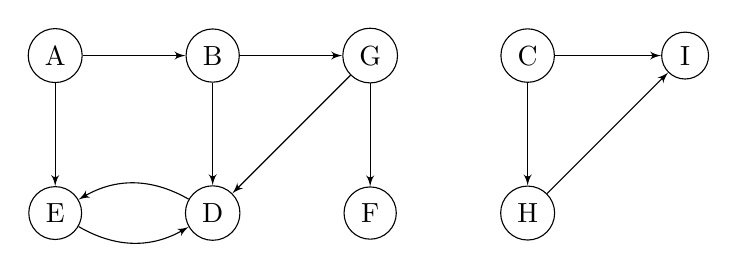
\begin{tikzpicture}\tikzset{vertex/.style = {shape=circle,draw,minimum size=1.5em}}\tikzset{edge/.style = {->,> = latex'}}\node[vertex] (a) at  (0,0) {A};\node[vertex] (b) at  (2,0) {B};\node[vertex] (d) at  (2,-2) {D};\node[vertex] (e) at  (0,-2) {E};\node[vertex] (g) at (4,0) {G};\node[vertex] (f) at (4,-2) {F};\node[vertex] (c) at (6,0) {C};\node[vertex] (i) at (8,0) {I};\node[vertex] (h) at (6,-2) {H};\draw[edge] (a) to (b);\draw[edge] (b) to (d);\draw[edge] (a) to (e);\draw[edge] (b) to (g);\draw[edge] (g) to (d);\draw[edge] (g) to (f);\draw[edge] (c) to (h);\draw[edge] (c) to (i);\draw[edge] (h) to (i);\draw[edge] (d)  to[bend right] (e);\draw[edge] (e) to[bend right] (d);\end{tikzpicture}}
%%%%% Don't Make Changes Above Here %%%%%

%%%%% Template Begins Here %%%%%

\def\Name{Ninh DO}  % Your name
\def\SID{25949105}  % Your student ID number
\def\Collabs{None} % Your collaborators here with a comma between each person's name. Write None if no collaborators. Don't leave blank.


\pagestyle{empty}
\begin{document}
\Title
%%%% Problem 1 Starts Here %%%%
\vspace{-2mm}\noindent\begin{mybox}{\begin{center}\textbf{\color{black}Problem 1: Million Dollar View}\end{center}}\end{mybox}\vspace{-2mm}
\begin{myboxot}\noindent\textbf{$\star\star\star\star$ Level}\end{myboxot} 

\noindent A $\$70$ million penthouse has recently been listed for sale in San Francisco. What used to be a perfect view of the Golden Gate Bridge has been marred by a recent development of towers and tech office buildings. Your job is to determine if the penthouse is worth the price, by obtaining the skyscrapers' outline. 
\vspace{3pt}

\noindent Suppose you are given the left and right positions of each of the buildings as well as the height in an array $A$ i.e. $[(lt_1,rt_1,ht_1),(lt_2,rt_2,ht_2),\cdots,(lt_n,rt_n, ht_n)]$. The left and right positions are on the $x$-axis and the height is on the $y$-axis. The output will be the key coordinates of the outline. These key coordinates are left points of the horizontal lines that form the outline. Thus we want the left point of the line as the $x$-coordinate and the height as the $y$-coordinate, i.e. $[(lt_1,ht_1),(lt_2,ht_2),\ldots]$. Input building positions are unsorted. See below for an example.

\hspace*{-0.5cm} 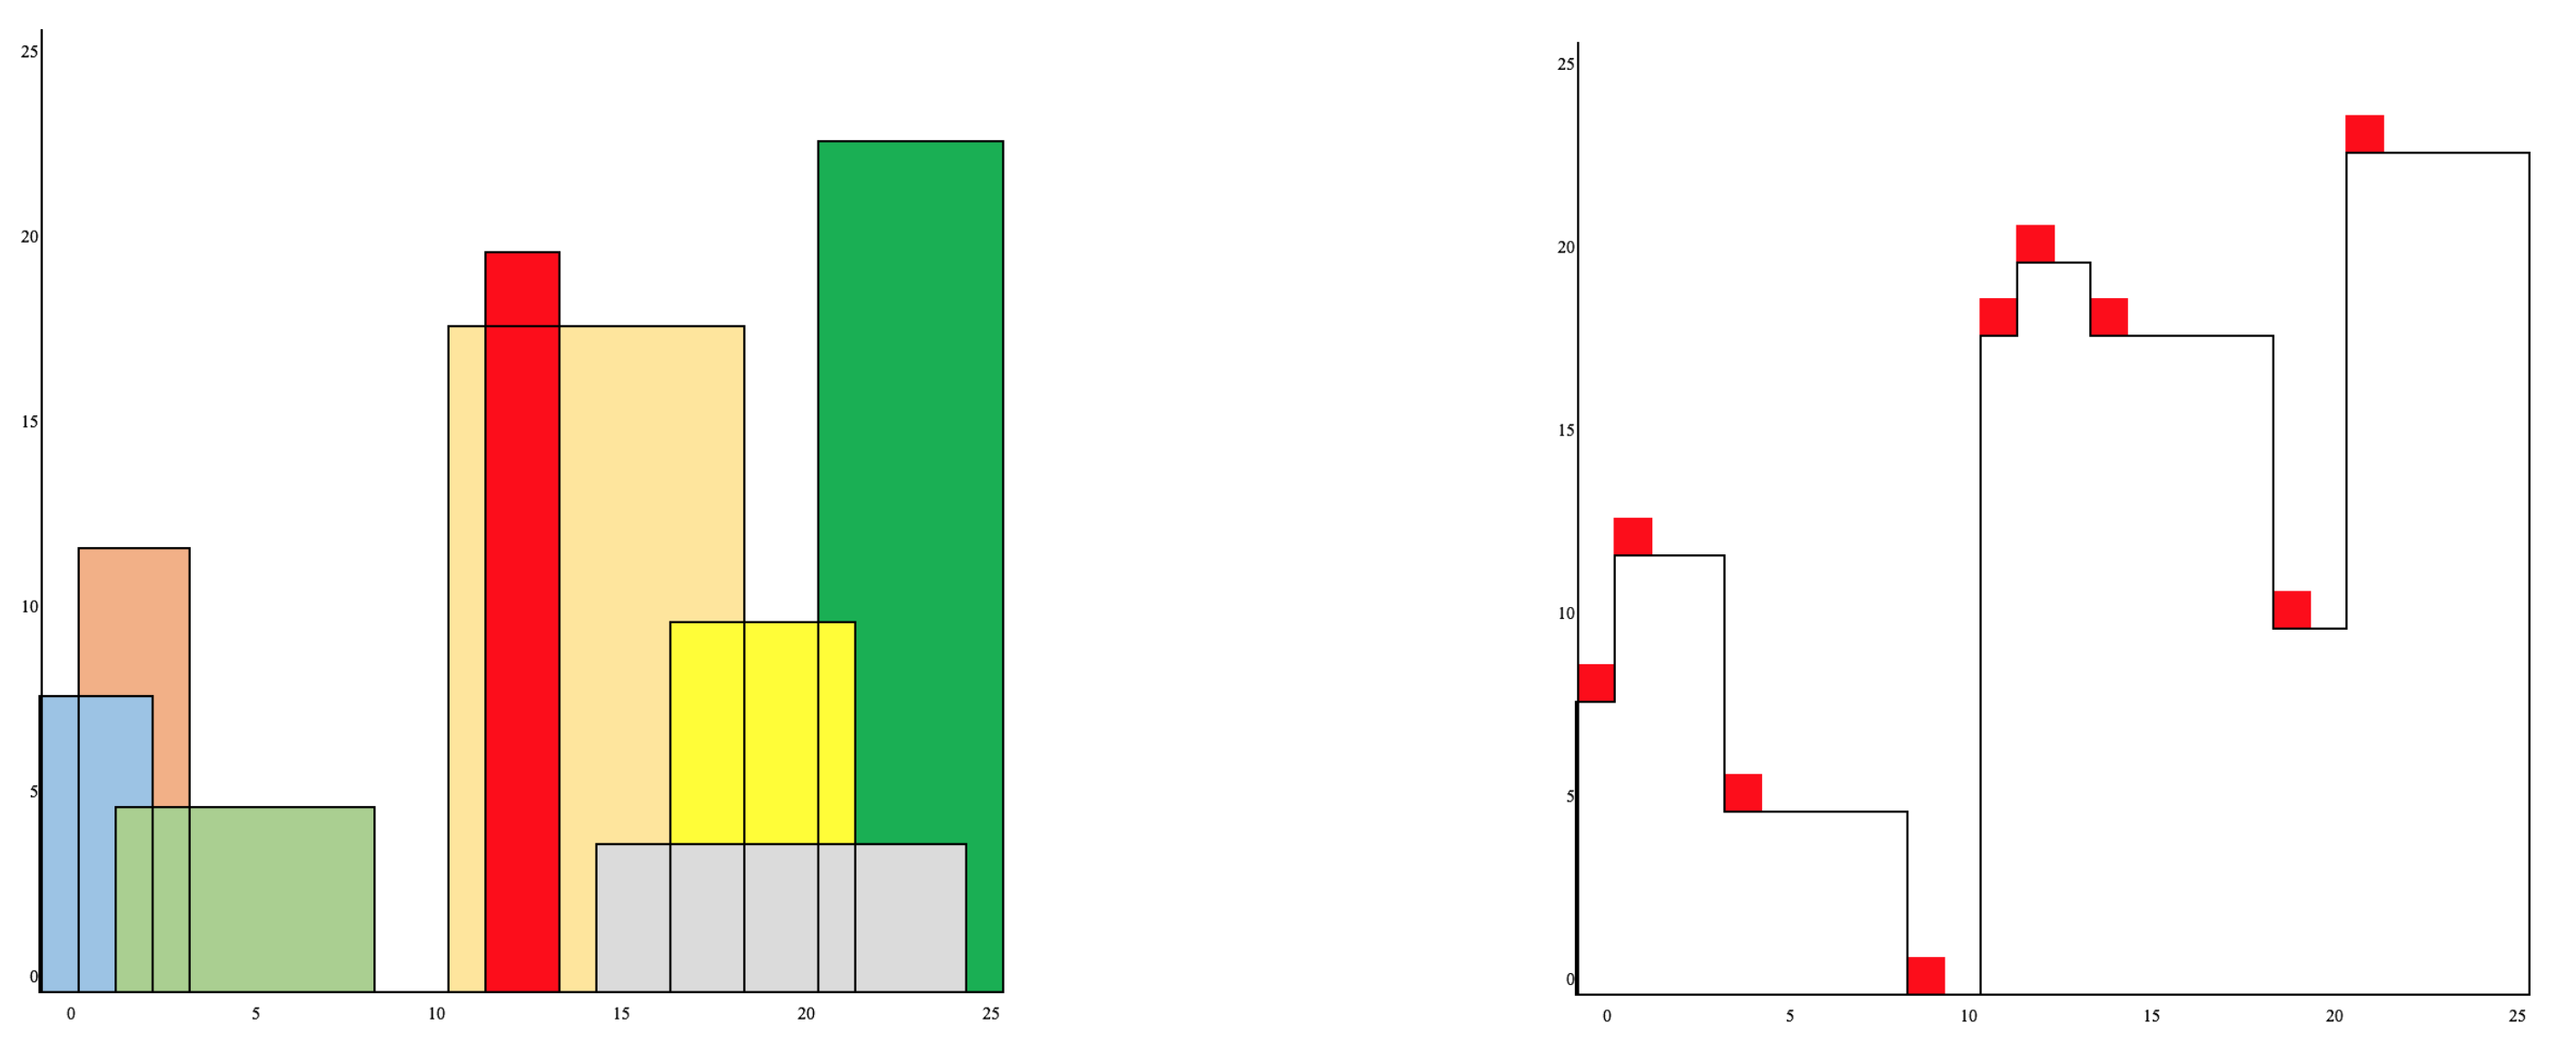
\includegraphics[width=\linewidth]{buildings}\\
\noindent Input buildings: $[(0,3,8),(1,4,12),(2,9,5),(11,17,18),(12,14,21),(15,25,4),(17,22,10),(21,26,23)]$ 

\noindent Output blocks: $[(0,8),(1,12),(4,5),(9,0),(11,18),(12,20),(14,18),(20,10),(22,23)]$
\vspace{3pt}

\noindent Design an efficient algorithm to compute the outline. \\

\BeginSolution % 1
% Solution Here
\\
\underline{\textbf{Main idea:}}\\
Apply Devide-and-Conquer to the problem: similar to merge-sort, to find the skyline of n building, we find skylines of two halves, each of which has $n/2$ buildings, then merge two skylines. To find skyline of each half of $n/2$ buildings, we divide it into two quaters, each of which has $n/4$ buildings, find skylines and merge them; so on. As a result, we have recursive algorithm with the base case to return the skylines of separate buildings.\\
\underline{\textbf{Pseudocode:}}\\
%
\begin{lstlisting}
def find_skyline(B):    # B is array of building positions and heights
	if len(B) == 1:
		return [(B[0][0],B[0][2]), (B[0][1],0)
	else
		skyline1 = find_skyline(B[0:n/2])
		skyline2 = find_skyline(B[n/2:n])
		skyline = merge_skyline(skyline1, skyline2)
		return skyline
		
def merge_skyline(sl1, sl2):    # we just cover all case for this function
	p1, p2 = 0, 0	# initialize two pointers to sl1 and sl2
	ret = []
	while p1 < len(sl1) and p2 < len(sl1):
		if p1 == 0 or p2 = 0:
			if sl1[p1][0] < sl2[p2][0]:
				ret.append((sl1[p1][0],sl1[p1][1]))
				p1 += 1
			else:
				ret.append((sl2[p2][0],sl2[p2][1]))
				p2 += 1	
		else:
			if sl1[p1][0] < sl2[p2][0]:
				if sl2[p2-1][0] < sl1[p1][0] and sl1[p1][1] < sl2[p2][1]:
					;
				else:
					ret.append((sl1[p1][0],sl1[p1][1]))
				p1 += 1
			else:
				if sl1[p1-1][0] < sl1[p1][0] and sl2[p2][1] < sl1[p1][1]:
					;
				else:
					ret.append((sl2[p2][0],sl2[p2][1]))
				p2 += 1
\end{lstlisting}
%
\underline{\textbf{Proof of correctness:}}\\
The algorithm is correct as long as the merge\_skyline method is correct. The merge\_skyline method is purely to check all the cases that two skylines at the pointers can overlap by moving the pointer forward and this is possible and to build one new skyline that cover the two old. This is feasible in constant time but we need not to go into detail for this. Therefore, the algorithm is correct.\\
\underline{\textbf{Runtime:}}\\
The recursive algorithm has the form $T(n)=2*T(n/2) + O(n)$. Using master theorem, the runtime is $O(n\log n)$
\EndSolution
%%%% Problem 1 Ends Here %%%%
\clearpage

%%%% Problem 2 Starts Here %%%%
\vspace{-2mm}\noindent\begin{mybox}{\begin{center}\textbf{\color{black}Problem 2: Majority Elements}\end{center}}\end{mybox}\vspace{-2mm}
\begin{myboxot}\noindent\textbf{$\star\star\star$ Level}\end{myboxot} 

\noindent An array $A[1\ldots n]$ is said to have a \textit{majority element} if more than half of its entries are the same. Given an array, the task is to design an efficient algorithm to tell whether the array has a majority element, and, if so, to find that element. The elements of the array are not necessarily from some ordered domain like the integers, and so there can be \textbf{no} comparisons of the form "if $A[i]>A[j]$?". (Think of the array elements as GIF files, say.) However, you \textit{can} answer questions of the form: "is $A[i] = A[j]$?" in constant time.
\vspace{5pt}

\noindent Can you give a linear-time algorithm?
\vspace{5pt}

\noindent (Hint: Here's a divide-and-conquer approach: 
\begin{itemize}
\item Pair up the elements of $A$ arbitrarily, to get about $n/2$ pairs
\item Look at each pair: if the two elements are different, discard both of them; if they are the same, keep just one of them
\item If $|A|$ is odd, there will be one unpaired element. What should you do with this element?
\end{itemize}
Show that after this procedure, there are at most $n/2$ elements left, and that they have a majority element if $A$ does.) \\
\BeginSolution % 2
% Solution Here
\\
\underline{\textbf{Main idea:}}
%
\begin{enumerate}[1.]
	\item Pair up the elements of $A$ arbitrarily, to get about $n/2$ pairs
	\item Look at each pair: if the two elements are different, discard both of them; if they are the same, keep just one of them
	\item If $|A|$ is odd, there will be one unpaired element, say A[k]. Loop through A to see if A[k] is majority element.
\end{enumerate}
%
\underline{\textbf{Pseudocode:}}
%
\begin{lstlisting}
original = A[:]    # copy of the array A
l = len(original)
n = len(A)
while n > 1:
	B = []
	for i = 0 --> (n - 1) by step 2:
		if A[i] == A[i+1]:
			B.append(a[i])
		end
	end
	if n is odd:
		count = 0
	 	for i = 0 --> (n - 1):
	 		if A[i] = A[n]:
	 			count++;
	 		end
	 	end
	 	if count > n/2:
	 		return A[n]
	 	end
	end
	A = B
	n = len(A)
end
ret = null
if len(A) == 1:                # important: reduced A has majority element 
	count = 0              # does not guarantee A has majority element, 
	for i = 0 --> (l - 1): # but reduced Ahas NO majority element confirm
	 	if A[0] = original[i]:    # A has NO majority element.
	 		count++;
	 	end
	end
	if count > l/2:
		ret = A[0]
end
return ret
\end{lstlisting}
%
\underline{\textbf{Proof of correctness:}}\\
We prove that after each $while$ loop, the number of elements is at most n/2. This is obvious, since the $for$ loop inside the $while$ loop jumps by step of 2 while B does not always append an element. Therefore, there are $int(n/2)$ $for$ iterations and $len(B) \leq n/2$\\
We prove that if $A$ has majority element, then $B$ has majority element: $B$ is a new array generated from $A$ after executing step 2 in the main idea part. Assume $A$ has majority element m, i.e. $count(m) > len(A)/2 > count(other\_elements)$. There are 2 cases:
%
\begin{enumerate}[1.]
	\item If we discard a non-identical pair, then $count(other\_elements)$ reduces by 2 if both elements are non-m, or $count(m)$ and $count(other\_elements)$ each reduces by 1 if it is the pair of m and non-m element. So either the reduce is fair or more towards $other\_elements$.
	\item For identical pairs, each will be reduced by half. Since the number of m-element idential pairs is larger than non-m element identical pair. Reducing by half still results in $count(m) > count(other\_elements)$
\end{enumerate}
%
Combining two cases, we always come up with $count(m) > count(other\_elements)$ after a cycle of reduction. Therefore, m is still majority element in B.\\
Now we have the clause: if $A$ has majority element, then $B$ has majority element. We can deduce that: if $B$ has NO majority element, then $A$ has NO majority element. This idea is reflected in the pseudocode when we check the length of $A$ after $while$ loop, that is if $len(A) == 0$ we return $null$. The existence of majority element in $B$ does not guarantee the existence of majority element in $A$ so we did loop through the original array to check. 
Both scenarios have been included in the pseudocose, so the algorithm is correct.\\
\underline{\textbf{Runtime:}}\\
For each $while$ loop, we implement $O(n)$ operations and reduce the array size by 2. The recursion equation is $T(n) = T(n/2) + O(n)$. Using master theorem, the runtime is $O(n)$
\EndSolution
%%%% Problem 2 Ends Here %%%%
\clearpage

%%%% Problem 3 Starts Here %%%%
\vspace{-2mm}\noindent\begin{mybox}{\begin{center}\textbf{\color{black}Problem 3: Triple Sum}\end{center}}\end{mybox}\vspace{-2mm}
\begin{myboxot}\noindent\textbf{$\star\star\star$ Level}\end{myboxot} 

\noindent Design an efficient algorithm for the following problem. We are given an array $A[0\ldots n-1]$ with $n$ elements, where each element of $A$ is an integer in the range $0\leqslant A[i]\leqslant 10n$. We are also given an integer $t$. The algorithm must answer the following yes-or-no question: do there exist indices $i,j,k$ such that $A[i]+A[j]+A[k]=t$?
\vspace{5pt}

\noindent Design $\mathcal{O}(n\log n)$ time algorithm for this problem.
\vspace{5pt}

\noindent \textit{Hint: define a polynomial of degree $\mathcal{O}(n)$ based upon $A$, then use FFT for fast polynomial multiplication.}\\
\BeginSolution % 3
% Solution Here
\\
\underline{\textbf{Main idea:}}
%
\begin{enumerate}[1.]
	\item Sort A using merge sort
	\item Define polynomial based on sorted A: $P = x^{A[0]} + x^{A[1]} + \dots + x^{A[n-1]}$, whose coefficient array is C.
	\item Use FFT for fast polynomial multiplication (aka FPM) to determine coefficients of $P^3$, called the coeffcient array $C3$.
	\item Inspect $C3[t]$. If $t$ is out of array dimension, or C3[t] == 0, then the answer to the problem is no. Otherwise, the answer is yes.
\end{enumerate}
%
\underline{\textbf{Pseudocode:}}
%
\begin{lstlisting}
A.sort()
m = max(A)    # polynomial order, actually m = A[n-1] since A is sorted
C = []        # initialize the coefficient array C of polynomial P
for i = 0 --> m:
	C[i] = 0
end
for j in A:
	C[j] += 1
end
C3 = FPM(FPM(C,C),C)  # polynomial multiplication using FFT, applying twice
ret = False
if t >= len(C3) || C3[t] == 0:
	return ret
else:
	ret = True
	return ret
end		
\end{lstlisting}
%
\underline{\textbf{Proof of correctness:}}\\
Consider polynomial:
%
\begin{equation*}
	P = x^{A[0]} + x^{A[1]} + \dots + x^{A[n-1]} \qquad (A\ sorted,\ m = A[n-1])
\end{equation*}
%
$P$ has order of $m=max(A)$ or $O(10n) \sim O(n)$, since $m\leq 10n$. Initially, the coefficients of these existing terms are 1, i.e. $C[A[i]] = 1$. If there are some $i, j$ such that $A[i] = A[j]$, then we can combine the equal terms into $C[A[i]] = 1 + 1$ omitting $x^{A[j]}$, i.e. accumulating the coefficient. The missing terms have coefficients 0. In general, we build P in the strict polynomial form for FFT purpose, i.e. order of terms in the series increases strictly by step 1 from 0 to $m$, and coefficients associated with missing terms are 0. Then:\\
%
\begin{equation*}
	P^3 = \sum\limits^{3m}_{l=0} c_l x^{A[i] + A[j] + A[k]} \qquad \text{index}\ l = A[i] + A[j] + A[k]
\end{equation*}
%
$P^3$ has terms to the power of all combinations of 3 elements from $A$, but the order of $P^3$ is just $3m$ since there are several triples whose sums are equal, so these terms are combined, i.e. their coefficients are accumulated to make larger coefficient. The key point is that the term of order $(A[i] + A[j] + A[k])$ is at the $(A[i] + A[j] + A[k])^{th}$ position in the zero-terms-including series and has coefficient $c_l$ with $l = A[i] + A[j] + A[k]$. It is simple because, like any regular polynomial $a_0 + a_1x + \dots + a_nx^n$, the term $a_ix^i$ lies at the $i^{th}$ position in the series and has coefficient $a_i$ (index $i$ of $a_i$ and exponent $i$ are the same).\\
Therefore, if we wanna check $t = A[i] + A[j] + A[k]$, we index $t$ into $C3$, which is the coefficient array of $P^3$. If $t>=len(C3)$ or $C3[t] == 0$, it means coefficient $c_t = 0$, i.e. there is no such triple making up t. Otherwise, there is.\\
\underline{\textbf{Runtime:}}
%
\begin{enumerate}[1.]
	\item Sorting A takes $\Theta(n\log n)$
	\item Defining polynomial P takes $\Theta(A[n-1])~$, i.e. $O(10n) \sim O(n)$, since $0\leq A[i]\leq 10n$
	\item FPM back and forth takes $O(n\log n)$, more precisely it take $O(30n\log 30n)$ but coefficient does not matter.
	\item Inspect $C3[t]$ take $O(1)$.\\
	The maximum runtime is $O(n\log n)$.
\end{enumerate}
%
\EndSolution
%%%% Problem 3 Ends Here %%%%
\clearpage

%%%% Problem 4 Starts Here %%%%
\vspace{-2mm}\noindent\begin{mybox}{\begin{center}\textbf{\color{black}Problem 4: Shortcut Question: Sherlock}\end{center}}\end{mybox}\vspace{-2mm}
\begin{myboxot}\noindent\textbf{$\star\star\star\star$ Level}\end{myboxot} 

\noindent Sherlock Holmes is trying to write a computer antivirus program. He starts by modeling his problem. He thinks of computer RAM as being a binary string $s_2$ of length $m$. He thinks of a virus as being a binary string $s_1$ of length $n<m$. His program needs to find all occurrences of $s_1$ in $s_2$ in order to get rid of the virus. Even worse, though, these viruses are still damaging if they differ slightly from $s_1$. So he wants to find all copies of $s_1$ in $s_2$ that differ in at most $k$ locations for arbitrary $k\leqslant n$.
\begin{enumerate}
\item Find an $\mathcal{O}(nm)$ algorithm for this problem. Give only the main idea; no four-part solution necessary.
\BeginSolution % 4a
% Solution Here
\\
\underline{\textbf{Main idea:}}\\
Run two $for$ loops, the outer one loops through 0 to $(m-1)-(n-1)$, we call the index $i$ the number of shifted bits of RAM. The inner loop goes through 0 to (n-1), we call the index $j$ the $j^{th}$ bit of virus and corresponding the $(i+j)^{th}$ bit of RAM.\\
For each time we shift bit (i.e. increasing $i$ by 1), we set a counter $count = 0$. Inside inner loop, we check if s2[i+j] == s1[j], where s2 and s1 are the bit strings of RAM and virus respectively. If they are not equal, increase counter by 1. At the end of i-iteration, if $count <= k$, i.e. there is either an occurrence of $s1$ in $s2$ or $s1$ only slightly differs from $s2$, then record the position i.\\
This algorithm runs in O(mn) time because we have two loops, one nested inside the other. Therefore, the runtime is the number of outter iterations multiplied by the number of inner iterations, i.e. $(m-n)*n \sim O(mn)$ 
\EndSolution
\item Find polynomials $p_1$ of degree $n-1$ and $p_2$ of degree $m-1$ such that the coefficient of $x^{n-1+i}$ of $p_1p_2$ is $n-2u(i)$ where $u(i)$ is the number of mismatched bits between $s_1$ shifted by $i$ and $s_2$. Show how to generate $p_1$ and $p_2$ in $\mathcal{O}(n+m)$ time. 
\BeginSolution % 4b
% Solution Here
\\
\underline{\textbf{Main idea:}}\\
Loop throught $s1$ of virus in backward order to form $p1$ and loop through $s2$ of RAM in forward order to form $p2$. While looping, if bit is 1, append 1 to $p$'s, if bit is 0, append -1 to $p$'s. Then $p1$ and $p2$ are the array of coefficients in ascending order of $x$ and each coefficient is either 1 or -1.\\
\underline{\textbf{Pseudocode:}}
%
\begin{lstlisting}
p1 = []
p2 = []
for i = 0 --> (n-1):
	if s1[(n-1)-i] == 0:
		p1[i] = -1
	else:
		p1[i] = 1
	end
end
for i = 0 --> (m-1):
	if s2[(m-1)-i] == 0:
		p2[i] = -1
	else:
		p2[i] = 1
	end
end
\end{lstlisting}
%
\underline{\textbf{Proof of correctness:}}\\
We prove that the polynomials $p_1$ of degree $n-1$ and $p_2$ of degree $m-1$ satisfy the condition that the coefficient of $x^{n-1+i}$ of $p_1p_2$ is $n-2u(i)$ where $u(i)$ is the number of mismatched bits between $s_1$ shifted by $i$ and $s_2$\\
First, let us consider two vectors $v_1$ and $v_2$ of 1 and -1 only. If $v_1$ and $v_2$ are identical, say $v_1 = v_2 = [1,-1,1,1,-1,1]$, then the dot product $p = v_1\cdot v_2 = 6 = len(v_1) = len(v_2)$, since the product of each element pair make 1. If they are differ in 1 position, say $v_1 = [1,-1,1,1,-1,1]$ and $v_2 = [1,-1,-1,1,-1,1]$, then the dot product $p = v_1\cdot v_2 = 1 + 1 - 1 + 1 + 1 + 1 = 6 - 2*1 = 4$, since the identical pair dots to 1, the opposite pair dot to -1.\\
We can generalize the rule as following: the dot product of two vectors of 1 and -1 is $n-2*k$ where $n$ is the length of vector and $k$ is the number of opposite element pairs. Proof is simple: given two n-element vectors $v_1$ and $v_2$ of 1 and -1 and they have $k$ opposite element pairs. Then the number of identical element pair is $n-k$. Their dot product $p = v_1\cdot v_2 = (n - k) - k = n - 2*k$, since identical pair makes 1, opposite pair make -1.\\
Returning to our problem, the string $s1$ has $n$ elements from 0 to $n-1$, the substring $ss_2$ has $n$ elements from $i$ to $n-1+i$ where $i$ is the number of bits that string $s_1$ is shifted. While the coefficient of $x^{n-1+i}$ is made from $s1[0]*s2[n-1+i] + s1[1]*s2[n-2+i] + s1[2]*s2[n-3+i] + \dots + s1[n-2+i]*s2[1] + s1[n-1+i]*s2[0]$, so we have to reverse $s2$ in order to ensure the correct implementation of dot product $s1*s2$\\
\underline{\textbf{Runtime:}}\\
Two loops are independent: First loop having $n$ iteration runs in $O(n)$ time, seconde loop having $m$ iteration runs in $O(m)$ time. The total runtime is $O(m+n)$.
\EndSolution
\item Find the main idea and runtime for an $\mathcal{O}(m\log m)$ algorithm for solving the problem for any $k$. Again, no four-part solution is necessary, but please clearly describe the algorithm and pseudocode if you think it will enhance our understanding of your solution.
\BeginSolution % 4c
% Solution Here
\\
\underline{\textbf{Main idea:}}\\
From question 4b, the coefficient of $x^{n-1+i}$ indirectly indicate the number of mismatch.\\
First, we formulate the polynomial $p1$ of degree $n-1$ from the reverse string $s1$ and the polynomial $p2$ of degree $m-1$ from the string $s2$ with the substitution of bit 1 by 1 and bit 0 by -1. Then we perform $p1p2=FPM(p1,p2)$. Subsequently, we inspect the coefficients of terms from power (n-1) to power (m-1). Those coefficients are equivalent to $n-2*u(i)$ where u(i) is the number of mismatched bits. We can compute $u(i) = (n - coeff)/2$. If u(i) < k, record $i$ which is the offset from (n-1).\\
We need not to care about the terms from power 0 to power (n-2), where s1 and s2 are not aligned.\\
This algorithm need: $O(n+m)$ for formulating $p1$ and $p2$, $O(m\log m)$ for $FPM(p1,p2)$, $O(m-n)$ for inspecting coefficients. The total runtime is $O(m\log m)$\\
\underline{\textbf{Pseudocode:}}
%
\begin{lstlisting}
Formulate p1, p2    # refer to pseudocode in 4b
p1p2 = FPM(p1,p2)
for i = 0 --> (m-n):
	coeff = p1p2[n-1+i]
	count = (n-coeff)
	if count <= k:
		record i
	end
end
\end{lstlisting}
%
\EndSolution
\end{enumerate}

%%%% Problem 4 Ends Here %%%%
\clearpage

%%%% Problem 5 Starts Here %%%%
\vspace{-2mm}\noindent\begin{mybox}{\begin{center}\textbf{\color{black}Problem 5: Graph Basics}\end{center}}\end{mybox}\vspace{-2mm}
\begin{myboxot}\noindent\textbf{$\star\star\star$ Level}\end{myboxot} 

\noindent For parts (a) and (b), refer to the figure below. For parts (c) through (f), please prove only for simple graphs; that is, graphs that do not have any parallel edges or self-loops.
\vspace{3pt}
\noindent\begin{center}\graph\end{center}
\begin{enumerate}
\item Run DFS at node $A$, trying to visit nodes alphabetically (e.g. given a choice between nodes $D$ and $F$, visit $D$ first).
\begin{itemize}
\item List the nodes in the order you visit them (so each node should appear in the ordering exactly once).
\item List each node with its pre- and post-number. The numbering starts from 1 and ends at 18.
\item Label each edge as \textbf{T}ree, \textbf{B}ack, \textbf{F}orward or \textbf{C}ross.
\end{itemize}
\BeginSolution % 5a
% Solution Here
\\
Order of visit: A  B  D  E  G  F    C  H  I\\
Pre- and post-number: A:1,12  B:2,11  C:13,18  D:3,6  E:4,5  F:8,9  G:7,10  H:14,17  I:15,16\\
Tree: A$\rightarrow$B, B$\rightarrow$D, B$\rightarrow$G, D$\rightarrow$E, G$\rightarrow$F, C$\rightarrow$H, H$\rightarrow$I\\
Back: E$\rightarrow$D\\
Forward: A$\rightarrow$E, C$\rightarrow$I\\
Cross: G$\rightarrow$D
\EndSolution
\item How many strongly connected components are there?
\BeginSolution % 5b
% Solution Here
\\
8 SCPs
\EndSolution
\item Let $|E|$ be the number of edges in a simple graph and $|V|$ be the number of vertices. Show that $|E|$ is in $\mathcal{O}\left(|V|^2\right)$.
\BeginSolution % 5c
% Solution Here
\\
Since one edge connects two vertices, so the maximum total number of edges $|E|$ is the number of combinations of two vertices out of total number of vertices $|V|$, i.e $|E|=C^{|V|}_2 of |V|=|V|*(|V|-1)/2=O(|V|^2)$
\EndSolution
\item For each vertex $v_i$, let $d_i$ be the \textit{degree} - the number of edges incident to it. Show that $\sum d_i$ must be even.
\BeginSolution % 5d
% Solution Here
\\
No any two vertices share the same end of an edge, and each edge is incident to 2 vertices in two direction. The number of edges incident to a vertice can be considered the number of ends of those edges. Since each set of ends of edges incident to each vertice does not overlap another, the total number of ends of all sets (or the total degree $\sum d_i$) is the total number of ends that all edges have. Each edges has two ends, so $\sum d_i = 2 * |E|$ which is an even number.
\EndSolution
\item An undirected graph $G$ is called \textit{bipartite} if we can separate its vertices into two subsets $A$ and $B$ such that every edge in $G$ must cross between $A$ and $B$. Show that a graph is bipartite if and only if it has no odd cycles.

\textit{Hint: Consider a spanning tree of the graph, which is a subset of the graph's edges which allow it to be a tree on all of its vertices.}
\BeginSolution % 5e
% Solution Here
\\
Consider a spanning tree of the graph, level of each node (vertex) is determined as following: root at level 0, chidren of root at level 1, children of children of root at level 2, so on. In general, each node is at the level equal to its distance from root. All vertices are divided into two groups: group A contains vertices at even levels, group B contains vertices at odd levels. The boundary between A and B cuts all edges of the tree.\\
If we add any edge the tree, it make a cycle. If edge has one end vertex in A, say at level $2*k$, one end vertex in B, say at level $2*l+1$, the number of nodes of cycles is $abs(2*l+1-2*k)+1$ which is an even cycle. If edge has two end vertices in A, say at levels $2*k$ and $2*l$, or two end vertices in B, say at level $2*k+1$ and $2*l+1$, the number of nodes of cycles is $abs(2*l-2*k)+1$ which is an odd cycle.\\
\underline{\textit{If the graph has no odd cycles, it is bipartite:}}\\
To prove this part, we just add edges to the tree above to make the graph, since we have only even cycles, those edges will have one end vertex in A and one end vertex in B, or they cross the boundary of A and B. Therefore, the graph is bipartite.\\
\underline{\textit{If the graph is bipartite, it has no odd cycles:}}\\
To prove this part, assume the graph has odd cycle, the edge of cycle that is not a part of tree must have two ends either in A or B. Otherwise, the cycle must be even. Since the graph has at least one edge totally lies either in A or B, it is not bipartite. Contradiction!\\
\EndSolution
\item A directed acyclic graph $G$ is \textit{semiconnected} if for any vertices $A$ and $B$ there is either a path from $A$ to $B$ or a path from $B$ to $A$. Show that $G$ is semiconnected if and only if there is a directed path that visits all of the vertices of $G$.
\BeginSolution % 5f
% Solution Here
\\
\underline{\textit{If there is a directed path that visits all of the vertices of $G$, $G$ is semiconnected:}}\\
To prove this part, take two arbitrary vertices of the graph, say A and B, they must be on the directed path p. Since they are on the path, there is a path p1, which is a sub-path of the directed path p, from A to B or from B to A. Since A and B are taken arbitrarily and they have a path, the graph is semiconnected by definition.\\
\underline{\textit{If $G$ is semiconnected, there is a directed path that visits all of the vertices of $G$:}}\\
To prove this part, assume there is NO directed path that visits all of the vertices of $G$, use DFS from a source to explore the graph. DFS will result in one or more branching trees. There is no path to go from one leaf of the trees to another leaf since the tree is directed, so the graph cannot be semiconnected. Contradiction!\\
\EndSolution
\end{enumerate}
%%%% Problem 5 Ends Here %%%%
\clearpage

%%%% Problem Redemption Starts Here %%%%
\vspace{-2mm}\noindent\begin{mybox}{\begin{center}\textbf{\color{black}Optional Redemption File}\end{center}}\end{mybox}\vspace{2mm}

\noindent Submit your \textit{redemption file} for Homework 1 here. If you looked at the solutions and took notes on what you learned or what you got wrong, include them here.

\end{document}
%%%%% Template Ends Here %%%%%